\documentclass{beamer}
\usepackage{amssymb,amsmath,mathrsfs}
\usepackage{catchfile,etoolbox}
\usepackage[PostScript]{../diagrams}
\usepackage{subfig}

\usepackage{epsfig,psfrag,epstopdf}

\newcommand{\sQ}{\mathcal{Q}}
\newcommand{\nc}{\mathit{nc}}

\usetheme{Szeged}

\usepackage{graphicx}
\graphicspath{{../figs/}}
\DeclareGraphicsExtensions{.pdf,.eps,.jpg,.png}

\usepackage{final_def}

\usepackage{media9}
\addmediapath{../prelim_def/videos}

\title[Energy Shaping]{Energy Shaping of Hybrid Systems\\via Control Lyapunov Functions}
\subtitle{Applications to Bipedal Walking\\ ---Final Examination}
\author{R. W. Sinnet}
\institute{Department of Mechanical Engineering\\ Texas A\&M University}
\date{Wednesday, October 15, 2014}


\begin{document}

\frame{\titlepage}

\begin{frame}
  \frametitle{Overview}
  \tableofcontents[sectionstyle=show,subsectionstyle=hide]
\end{frame}

\ifdefstring{\PRELIMSECA}{1}{\section{Introduction}
\showtoc

\subsection{Motivation}

\begin{frame}[t]
  \frametitle{Goal}
  \begin{block}{Main Goal}
    Develop methods for achieving bipedal robotic walking in an elegant manner by fusing complementary control schemes.
  \end{block}
    \begin{columns}
    \begin{column}{.333\textwidth}
      \begin{figure}
        \centering
        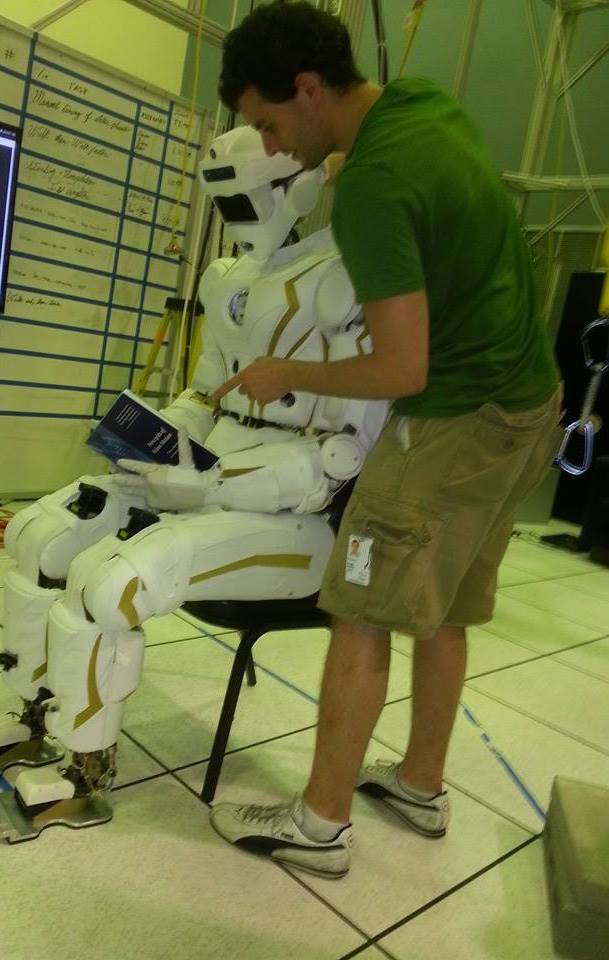
\includegraphics[height=4.0cm]{sinnet_valkyrie}
      \end{figure}
    \end{column}
    \begin{column}{.333\textwidth}
      \begin{figure}
        \centering
        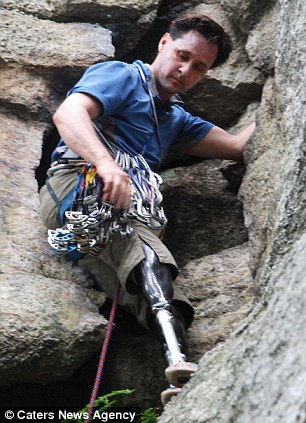
\includegraphics[height=4.0cm]{hugh_herr_climbing}
      \end{figure}
    \end{column}
    \begin{column}{.333\textwidth}
      \begin{figure}
        \centering
        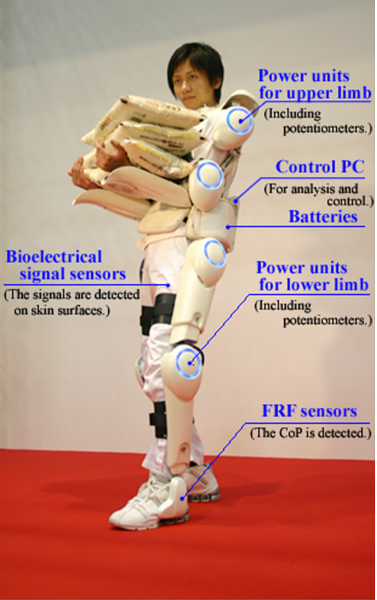
\includegraphics[height=4.0cm]{exoskeleton}
      \end{figure}
    \end{column}
  \end{columns}
\end{frame}

\begin{frame}[t]
  \only<1> {
    {\Large \bf Biomechanics}
    \begin{itemize}
    \item
      D.~A. Winter, {\em Biomechanics and Motor Control of Human Movement}, 2nd ed., New York: Wiley-Interscience, 1990.\\
    \item
      J. Perry and J. Burnfield, Gait Analysis: Normal and Pathological Function, 2nd ed., Thorofare: Slack Inc., 2010.\\
    \end{itemize}
  }
  \only<2,3> {
    \textcolor{gray}{\Large \bf Biomechanics}\\[1mm]
  }

  \only<2> {
    {\Large \bf Reduction-Based Control}
    \begin{itemize}
    \item
      A.~D. Ames et al., {\em On the Geometric Reduction of Controlled Three-Dimensional Bipedal Robotic Walkers}, in 3rd Workshop on Lagrangian and Hamiltonian Methods for Nonlinear Control (LHMNL'06), Nagoya, Japan, Jul. 2006.\\
    \item
      R.~W. Sinnet et al., {\em 3D Bipedal Walking with Knees and Feet: A Hybrid Geometric Approach}, in 48th IEEE Conference on Decision and Control, Shanghai, P. R. China, Dec. 2009.
    \item
      R~.W. Sinnet and A.~D. Ames, {\em Bio-Inspired Feedback Control of Three-Dimensional Humanlike Bipedal Robots}, in Journal of Robotics and Mechatronics, special issue on {\em Focused Areas and Future Trends in Bio-Inspired Robots}, Aug. 2012.

    \end{itemize}
  }
  \only<1,3> {
    \textcolor{gray}{\Large \bf Reduction-Based Control}\\[1mm]
  }

  \only<3> {
    {\Large \bf Human-Inspired Control}
    \begin{itemize}
    \item
      A.~D. Ames, {\em First Steps Toward Automatically Generating Bipedal Robotic Walking from Human Data}, in 8th International Workshop on Robotic Motion and Control, Gron{\'o}w, Poland, Jun. 2011.
    \item
      R.~W. Sinnet et al., {\em A Human-Inspired Hybrid Control Approach to Bipedal Robotic Walking}, in 18th IFAC World Congress (IFAC 2011), Milan, Italy, Sep. 2011.
    \item
      R.~W. Sinnet et al., {\em A Human-Inspired Framework for Bipedal Robotic Walking Design}, International Journal of Biomechatronics and Biomedical Robotics, Jan. 2014.
    \end{itemize}
  }
  \only<1,2> {
    \textcolor{gray}{\Large \bf Human-Inspired Control}
  }

\end{frame}

\begin{frame}[t]
  \frametitle{History}
  \begin{columns}

    \begin{column}{.24\textwidth}
      \textcolor{blue}{Passive Walking:}
      \begin{figure}
        \centering
        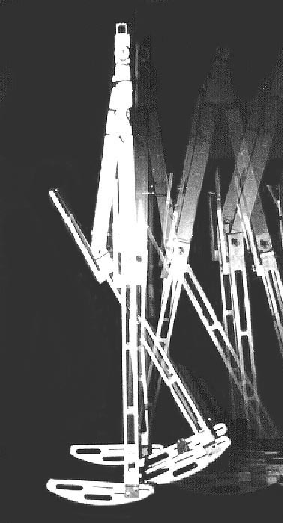
\includegraphics[height=4.5cm]{bipeds_ruina}
      \end{figure}
    \end{column}

    \begin{column}{.24\textwidth}
      \textcolor{blue}{Passivity-Based Control:}
      \begin{figure}
        \centering
        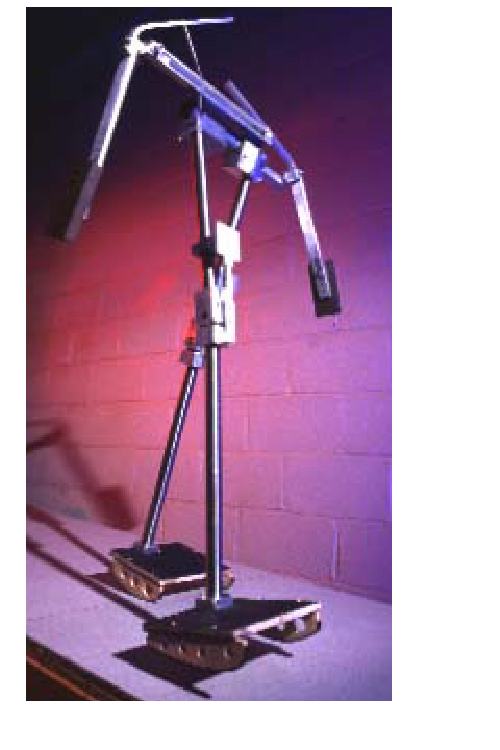
\includegraphics[height=4.5cm]{bipeds_collins}
      \end{figure}
    \end{column}

    \begin{column}{.24\textwidth}
      \textcolor{blue}{Hybrid Zero Dynamics:}
      \begin{figure}
        \centering
        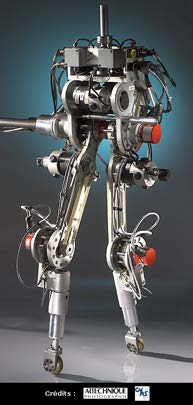
\includegraphics[height=4.5cm]{bipeds_grizzle}
      \end{figure}
    \end{column}

    \begin{column}{.24\textwidth}
      \textcolor{blue}{Human-Inspired Control:}
      \begin{figure}
        \centering
        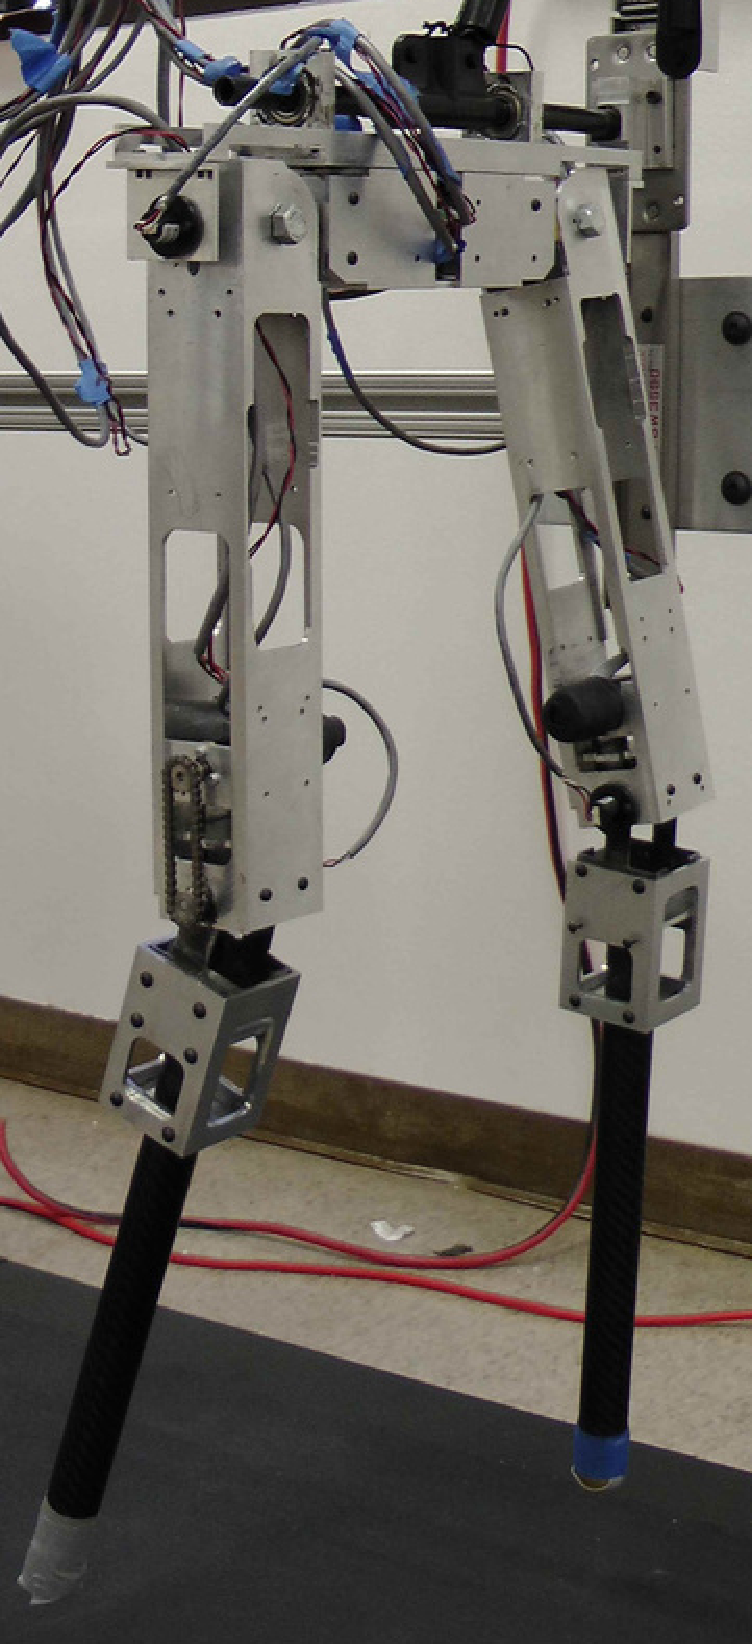
\includegraphics[height=4.5cm]{bipeds_ames}
      \end{figure}
    \end{column}

  \end{columns}
\end{frame}
}{}
\ifdefstring{\PRELIMSECB}{1}{\section{Mechanics}
\showtoc

\subsection{Hybrid Systems}
\begin{frame}[t]
  \frametitle{Bipedal Models}
  \begin{figure}
    \centering
    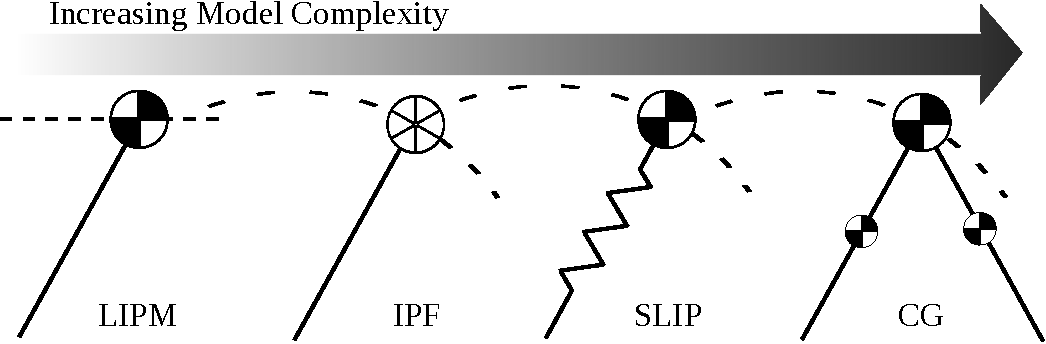
\includegraphics[width=.9\textwidth]{biped-models}
  \end{figure}
  \begin{itemize}
  \item Bipedal locomotion has been studied with a variety of models.
  \item Pendulum models consider massless legs with no impacts.
  \item Kinematic chains are markedly more complex than pendula.
  \end{itemize}
\end{frame}

\begin{frame}[t]
  \frametitle{Modeling Hybrid Systems}
  \begin{columns}
    \begin{column}{.63\textwidth}
      \begin{definition}
        A \alert{hybrid control system} is a tuple \vspace{-.3cm}
        $$\HCS = \hcsystem, \vspace{-.4cm}$$
        where
        \begin{itemize}
        \item
          $\Domain \subset \X$ is the \blue{domain of admissibility} with state space $\X$,
        \item
          $\ControlSet$ is a set of \blue{admissible controls},
        \item
          $\Guard$ is a \blue{guard} or \blue{switching surface},
        \item
          $\ResetMap$ is a smooth \blue{reset map},
        \item
          $(\xf, \xg)$ is a \blue{control system} on $\Domain$: \vspace{-3mm}
          \begin{align*}
            \dx = \xf(\x) + \xg(\x) \, \uu.
          \end{align*}
        \end{itemize}
      \end{definition}
    \end{column}
    \begin{column}{.4\textwidth}
      \begin{figure}    
        \centering
        \def\svgwidth{.8\columnwidth}
        \input{../figs/simple_hybrid_system.eps_latex}
      \end{figure}
      \vspace{-1em}
      A \alert{simple hybrid system}:\vspace{-.5em}
      $$\HS = \hsystem$$
    \end{column}
  \end{columns}
\end{frame}

\begin{frame}[t]
  \frametitle{Lagrangian Systems}
  Mechanical systems are defined by:
  \begin{itemize}
  \item Kinetic energy, $T : T\sQ \to \Rnn$,\\
  \item Potential energy, $U : \sQ \to \R$,
  \end{itemize}
  which together comprise the Lagrangian,
  \begin{align*}
    \Lagrangian\argsqdq = T\argsqdq - U\argsqdq.
  \end{align*}
  Dynamical motion in such a system with external forcing $\mathcal{F} = B\argsq u$ is governed by the Euler--Lagrange equation:
  \begin{align*}
    \frac{d}{dt} \pd{\Lagrangian}{\dq} - \pd{\Lagrangian}{\q} = B\argsq u.
  \end{align*}
\end{frame}

\begin{frame}[t]

  \frametitle{Swing Phase Dynamics}
  \begin{columns}
    \begin{column}{.55\textwidth}
      For Lagrangian $\Lagrangian$ with coordinates
      \begin{align*}
        \x = \argsqdq \in T\ConfigurationSpace,
      \end{align*}
      the dynamic model has the form
      \begin{align*}
        \M\argsq \, \ddq + \C\argsqdq \, \dq + \G\argsq = \B\argsq \, \uu,
      \end{align*}
      or $\dx = \xf\argsqdq+ \xg\argsq \, \uu,$ with
      \begin{align*}
        \xf\argsqdq &= \left(\!\!\begin{array}{c}
            \dq\\
            \M^{-1}\argsq (-\C\argsqdq \, \dq - \G\argsq)
          \end{array}\!\!\right),\\
        \xg(\q) &= \left(\!\!\begin{array}{c}
            \mathbf{0}_{m \times m}\\
            \M^{-1}(\q) \B(\q)
          \end{array}\!\!\right).
      \end{align*}
    \end{column}\!\!
    \begin{column}{.45\textwidth}
      \begin{figure}
        \centering
        \vspace{-10mm}
        \caption{Physical configuration}
        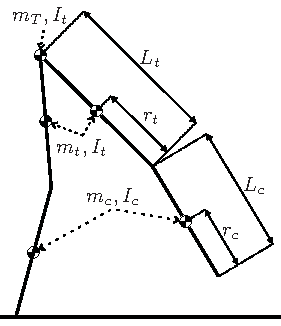
\includegraphics[width = 1.0\columnwidth]{pointfoot_robot_config}
      \end{figure}
    \end{column}
  \end{columns}
\end{frame}

\begin{frame}[t]
  \frametitle{Impact Dynamics}
  Introduce extended coordinates $\qe = (X, \q) \in \mathrm{SE}(3) \times \ConfigurationSpace$ which contains the kinematics of a reference point on the robot. Angular momentum balance based on H{\"u}rm{\"u}zl{\"u} and Marghitu:
  \begin{massump}
    \begin{itemize}
    \item Rigid-body plastic impacts
    \item Enough friction to prevent slipping
    \item Motors do not produce impulses
    \item No instantaneous change in configuration, i.e., $\qe^{-} = \qe^{+}$
    \end{itemize}
  \end{massump}
  Under these assumptions, the discrete dynamics satisfies
  \begin{align*}
    \left[\begin{array}{c c}
        \D_{e}(\qe) & -\Jacobian^{T}(\qe)\\
        \Jacobian(\qe) & \mathbf{0}_{3 \times 3}
      \end{array}\right]
    \left[\begin{array}{c}
        \dq^{+}\\
        \delta F(\qe, \dqe)
      \end{array}\right]
    = \left[\begin{array}{c c}
        \D_{e}(\qe) \, \dqe^{-}\\
        \mathbf{0}_{3}
      \end{array}\right].
  \end{align*}
\end{frame}

\subsection{Solutions to Hybrid Systems}
\begin{frame}[t]
  \frametitle{Hybrid Flows}
  A \alert{hybrid flow} of $\HS$ is a tuple
  \begin{align*}
    \chi^{\HS} = \left( \Delta, \mathscr{I}, \mathscr{C} \right),
  \end{align*}
  \vspace{-2em}
  \begin{itemize}
  \item $\Delta = \{0, 1, 2, \ldots\} \subseteq \Nat$ is a finite or infinite \blue{indexing set},
  \item $\mathscr{I} = \{I_{i} \}_{i \in \Delta}$ is a \blue{hybrid interval} where $I_{i} = [\tau_{i}, \tau_{i + 1}]$,
  \item $\mathscr{C} = \{c_{i} \}_{i \in \Delta}$ is a \blue{collection of solutions} of $\xf$, i.e., ${\dot c}_{i}(t) = \xf(c_{i}(t))$ $\forall i \in \Delta$.
  \end{itemize}

  \only<1>{
    \vspace{-1em}
    \begin{figure}
      \centering
      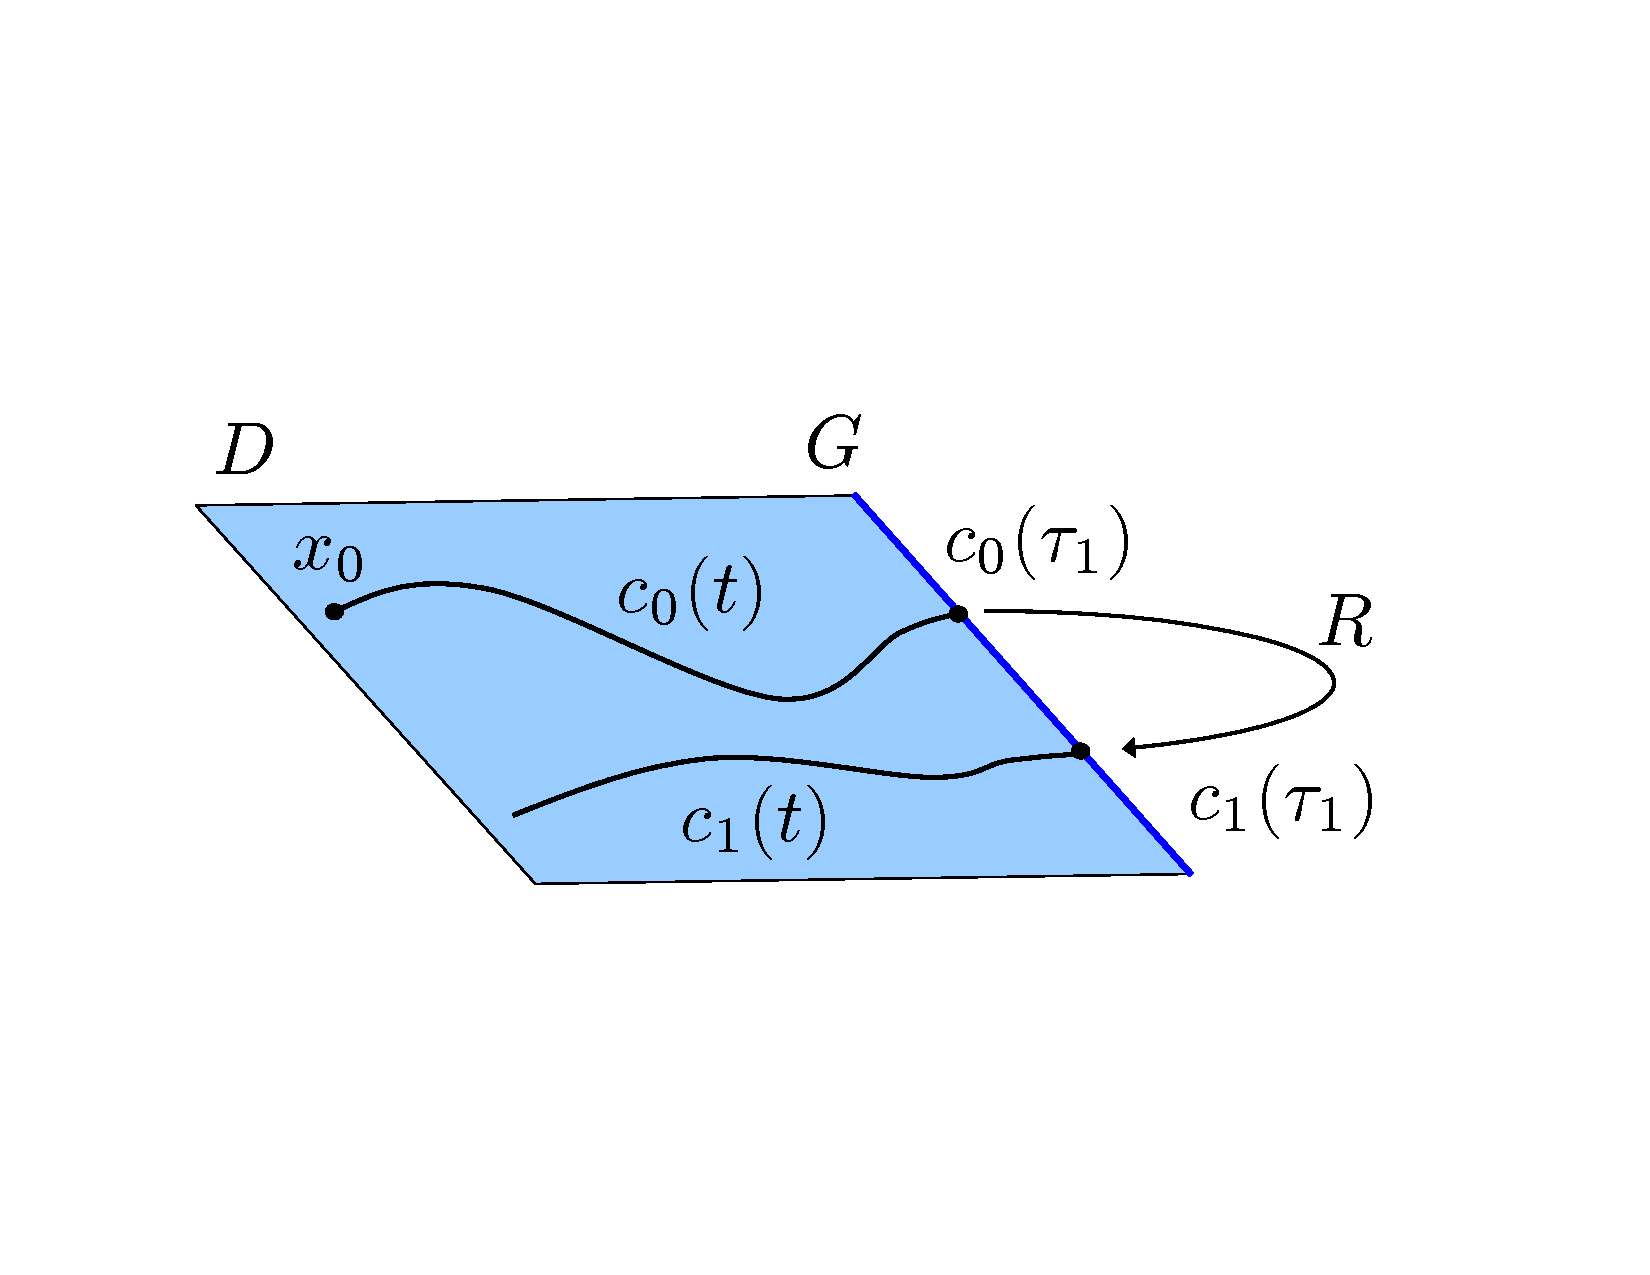
\includegraphics[width=0.5\columnwidth]{hybridflow}
    \end{figure}
    \vspace{-1em}
  }

  \only<2>{
    In addition, for every $i, i + 1 \in \Delta$, it is required that
    \begin{enumerate}
    \item $c_{i}(\tau_{i+1}) \in G$ and
    \item $\Delta(c_{i}(\tau_{i+1})) = c_{i+1}(\tau_{i+1})$
    \end{enumerate}
  }
\end{frame}


\begin{frame}[t]
  \frametitle{Periodic Orbits}
  \begin{figure}    
    \centering
    \def\svgwidth{.45\columnwidth}
    \input{../figs/hybrid_periodic_orbit.eps_latex}
    \caption{A hybrid periodic orbit. Stability is ascertained using the method of Poincar\'e.}
  \end{figure}
\end{frame}

\begin{frame}[t]
  \frametitle{Conservative Systems}
  For a conservative system, total energy is conserved; i.e.:
  \begin{align*}
    \Ec &= T\argsqdq + U\argsq\\
    &= \E(q(0), \dot q(0)) = \E_{0}
  \end{align*}
  Dynamical motion for such a system relies on the interplay between kinetic and potential energy, which is expressed in the Euler-Lagrange equation,
  \begin{align*}
    \frac{d}{dt} \pd{\Lagrangian}{\dq} - \pd{\Lagrangian}{\q} = 0.
  \end{align*}
\end{frame}


\begin{frame}[t]
  \frametitle{The Simplest Example: Passive Compass-Gait Biped}
  \only<1>{
    \begin{columns}
      \column{1.5in}
      Dynamic Model:
      \begin{align*}
        \M\argsq \ddot q + \CG\argsqdq = 0
      \end{align*}
      Control Law:
      \begin{align*}
        \uu = 0.
      \end{align*}
      \column{1.5in}
      \begin{figure}%width=1.0\columnwidth,
        
        \centering
        \def\svgwidth{1.0\columnwidth}
        \input{../figs/cg2d-slope-model.eps_latex}
        \vspace{-2em}
        \caption{Compass-gait biped falling down a slope.}
      \end{figure}
    \end{columns}
  }

  \only<2>{
    \begin{figure}
      \includemedia[
      % width=1.0\columnwidth,
      % height=0.5625\columnwidth,
      %width=1.0\columnwidth,
      %height=0.5\columnwidth,
      width=.9\columnwidth,
      height=0.45\columnwidth,
      addresource=cg2d_slope.mp4,
      activate=pageopen,
      flashvars={source=cg2d_slope.mp4&loop=true&autoPlay=true}
      ]{}{VPlayer9.swf}
      \caption{Stable passive gaits can be found for a range of slopes.}
    \end{figure}    
  }

  \only<3>{
    \begin{figure}
      \centering
      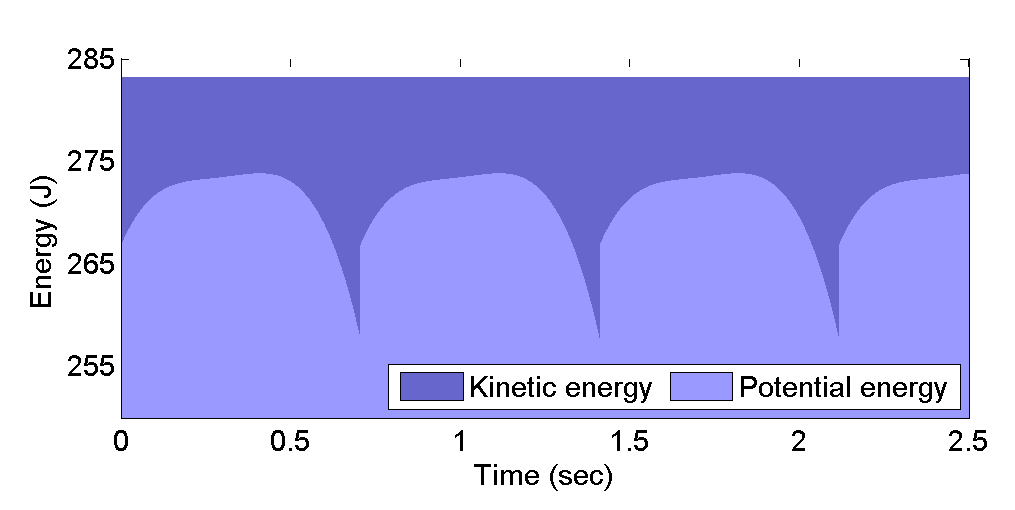
\includegraphics[width=1.0\columnwidth]{energy_cg2d_slope_model}
      \caption{Energy is exchanged between kinetic and potential in form.}
    \end{figure}    
  }
\end{frame}


\begin{frame}[t]
  \frametitle{Nonconservative Systems}
  For a nonconservative system, energy flows out of the system at a rate of $F_{\nc} \cdot dq$. Thus, the following quantity is conserved:
  \begin{align*}
    \Ec &= T\argsqdq + U\argsq - \int_{t_{0}}^{t} \! F_{\nc} \cdot \frac{dq}{d\tau} \ d\tau\\
    &= \E(q(0), \dot q(0)) = \E_{0}
  \end{align*}
  This equation expresses the interplay between kinetic and potential energy and the flow of energy into and out of the system.
\end{frame}


\begin{frame}[t]
  \frametitle{Example: Active Compass-Gait Biped}
  \only<1>{
    \begin{columns}
      \column{1.5in}
      Dynamic Model:
      \begin{align*}
        \M\argsq \ddq + \CG\argsqdq = \B\argsq \uu.
      \end{align*}
      Controlled Symmetries:
      \begin{align*}
        \uu &= \G\argsq - G(\Psi_{\gamma}\argsq)
      \end{align*}
      where $\Psi : \S \times \R \to \sQ$ rotates the frame of gravity by $\gamma$.

      \column{1.5in}
      \begin{figure}
        \centering
        \def\svgwidth{1.0\columnwidth}
        \input{../figs/cg2d-2link-model.eps_latex}
        \vspace{-2em}
        \caption{Compass-gait biped with Controlled Symmetries.}
      \end{figure}
    \end{columns}
  }
  \only<2>{
    \begin{figure}
      \includemedia[
      % width=1.0\columnwidth,
      % height=0.5625\columnwidth,
      width=.9\columnwidth,
      height=0.45\columnwidth,
      addresource=cg2d_2link_simulation.mp4,
      activate=pageopen,
      flashvars={source=cg2d_2link_simulation.mp4&loop=true&autoPlay=true}
      ]{}{VPlayer9.swf}
      \caption{Passive downhill gaits can be translated to flat ground with Controlled Symmetries.}
    \end{figure}    
  }
  \only<3>{
    \begin{figure}
      \centering
      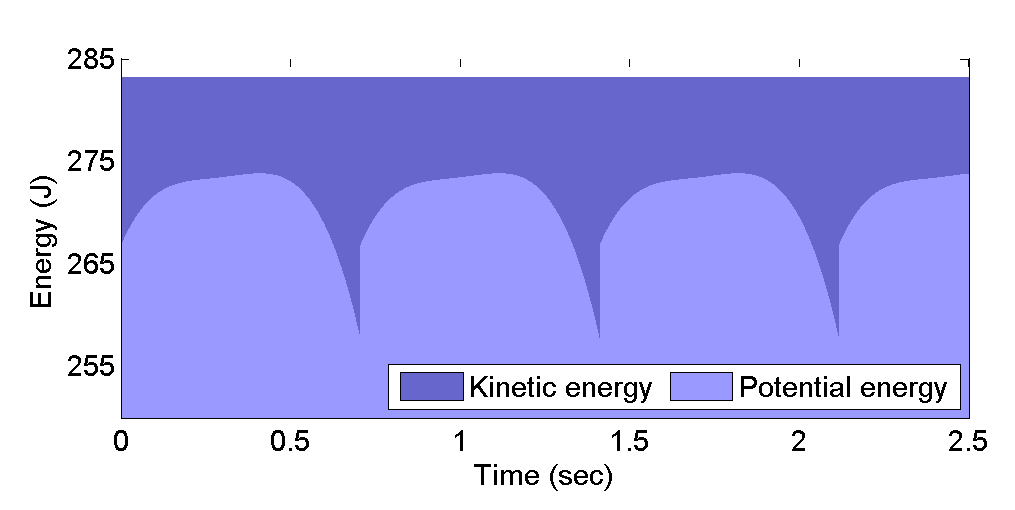
\includegraphics[width=1.0\columnwidth]{energy_cg2d_slope_model}
      \caption{Energy of the shaped system is conserved.}
    \end{figure}    
  }
\end{frame}

\begin{frame}[t]
  \frametitle{Example: 3-Link Biped}
  \only<1>{
    \begin{columns}
      \column{1.5in}
      Dynamic Model:
      \begin{align*}
        \M\argsq \ddq + \CG\argsqdq = \B\argsq \uu
      \end{align*}
      Control Law:
      \begin{align*}
        \uu &= \G\argsq - \G(\Psi\argsq)\\
        \uu_3 &=-k_{d} (\dot \vartheta_{T}^{a})\\
        &\hspace{1.8em} -k_{p} (\vartheta_{T}^{a} - \vartheta_{T}^{d})
      \end{align*}
      \column{1.5in}
      \begin{figure}
        \centering
        \def\svgwidth{1.0\columnwidth}
        \input{../figs/cg2d-3link-model.eps_latex}
        \vspace{-2em}
        \caption{3-link biped configuration.}
      \end{figure}
    \end{columns}
  }

  \only<2>{
    \begin{figure}
      \centering
      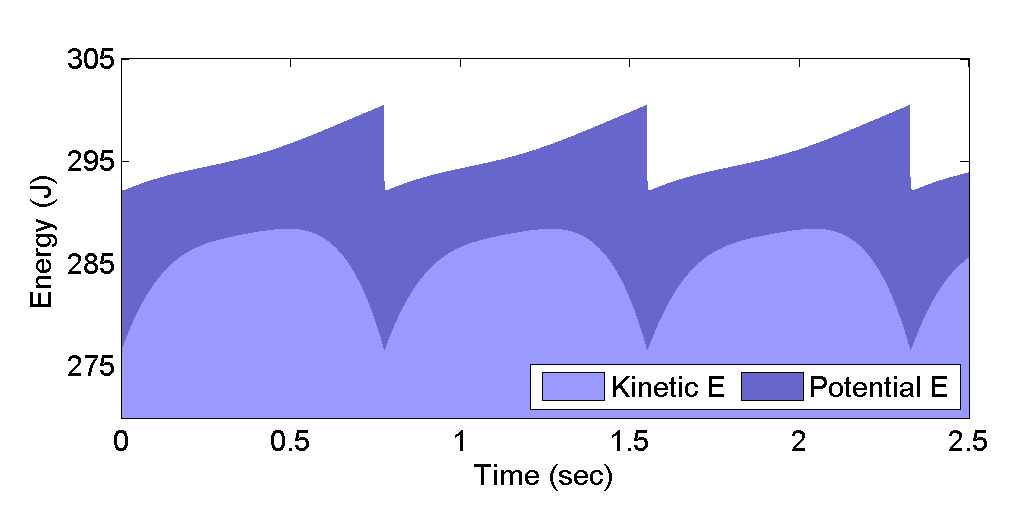
\includegraphics[width=1.0\columnwidth]{energy_cg2d_3link}
      \caption{Energy is not conserved as the controller injects energy.}
    \end{figure}
  }

  \only<3>{
    \begin{figure}
      \includemedia[
      %width=1.0\columnwidth,
      %height=0.5\columnwidth,
      width=.9\columnwidth,
      height=0.45\columnwidth,
      addresource=cg2d_3link_simulation.mp4,
      activate=pageopen,
      flashvars={source=cg2d_3link_simulation.mp4&loop=true&autoPlay=true}
      ]{}{VPlayer9.swf}
      \caption{Stable passive gaits can be found for a range of slopes.}
    \end{figure}
  }
\end{frame}
}{}
\ifdefstring{\PRELIMSECC}{1}{\section{Energy Shaping}
\showtoc

\subsection{Energy Shaping with Control Lyapunov Functions}

\begin{frame}[t]
  \frametitle{Motivation}
  \begin{block}{Main Question}
    Can we use an understanding of energy exchange to improve robustness  of
    periodic orbits in hybrid mechanical systems?
  \end{block}

  \begin{block}{Observations}
    \begin{itemize}
    \item Numerous control design schemes exist for stabilizing hybrid mechanical
      systems to periodic orbits.
    \item Some controllers produce good behavior locally but lack robustness.
    \item Periodic orbits have associated energy functions with level sets which
      are invariant under the orbits.
    \end{itemize}
  \end{block}
\end{frame}

\begin{frame}[t]
  \frametitle{Overview}
  \begin{block}{Main Idea}
    Add robustness to a periodic behavior by imposing convergence on a conserved
    energy function, $\Ec : \x \to \R$, to a level set which is known to be
    invariant under the system dynamics.
  \end{block}
  
  \begin{block}{Control Objective}
    Choose control input $\mu\arx$ such that $\| \mu\arx \|$ is minimized and
    $\Ec\arxt \to \Eref$ as $t \to \infty$.
  \end{block}

  \begin{block}{Exponential Convergence}
    To achieve exponential stabilization, $\Ec\arxt$ should satisfy\vspace{-.4em}
    \begin{align*}
      \Ec\arxt \leq \Ec\arxzero e^{-\beta t} \mbox{ for } t \geq 0, \beta > 0.
    \end{align*}
  \end{block}
\end{frame}

\begin{frame}[t]
  \frametitle{Conserved Energy Functions}
  \only<1> {
    \begin{block}{Conservative Systems}
      A conservative system with state space $\x = \argsqdq$ is modeled as
      \begin{align*}
        \HCSbar = \left\{
          \begin{array}{l l}
            \left.\begin{array}{r c l}
                \hspace{.58em}\dx &=& \xfbar\argsqdq + \xgbar\argsq \, \uu
              \end{array}\right\}  & \mbox{if } \argsqdq \in \D \setminus \S,\\
            \left. \begin{array}{r c l}
                \qp &=& \Deltaq\argsqm\\
                \dqp &=& \Deltadq\argsqdqm
              \end{array} \right\} & \mbox{if } \argsqdq \in \S,
          \end{array}\right.
      \end{align*}
      where $\xfbar\argsqdq := \xf\argsqdq$ and $\xgbar\argsq := \xg\argsq$ for
      notational clarity. Total energy is conserved through the continuous
      dynamics, i.e.,
      \begin{align*}
        \Ec\argsqdq := T\argsqdq + U\argsq.
      \end{align*}
    \end{block}
  }

  \only<2> {
    \begin{block}{Nonconservative Systems}
      To properly handle the flow of energy due to $\vv\argsqdq$, define a storage
      function, $\W$, which obeys the differential equation
      \begin{align*}
        d\W = \vfR\argsqdq \, dt = \left( \B\argsq \, \vv\argsqdq \right)^{T}
        \frac{d\q}{dt}\art \, dt.
      \end{align*}
      Using $\W$, augment the state space, i.e., $\x := (\q, \dq, \W)$, and the vector
      fields (subsuming $\vv\argsqdq$ under $\xfbar\argsqdq$), i.e, 
      \begin{align*}
        \xfbar\argsqdq := \left(\begin{array}{c}
            \xf\argsqdq + \xg\argsq \, \vv\argsqdq\\
            \vfR\argsqdq
          \end{array}\right), &&
        \xgbar\argsq := \left(\begin{array}{c}
            \xg\argsq\\
            \boldzero
          \end{array}\right).
      \end{align*}
    \end{block}
  }
  \only<3> {
    \begin{block}{Nonconservative Systems}
      Use the augmented state to define the hybrid control system
      \begin{align*}
        \HCSbar = \left\{
          \begin{array}{l l}
            \left.\begin{array}{r c l}
                \hspace{1.15em}\dx &=& \xfbar\argsqdq + \xgbar\argsq \, \uu
              \end{array}\right\}  & \mbox{if } \argsqdq \in \D \setminus \S,\\
            \left. \begin{array}{r c l}
                \qp &=& \Deltaq\argsqm\\
                \dqp &=& \Deltadq\argsqdqm\\
                \Wp &=& \DeltaW = 0
              \end{array} \right\} & \mbox{if } \argsqdq \in \S.
          \end{array}\right.
      \end{align*}
      For such a system, the following quantity is conserved:
      \begin{align*}
        \Ec\argsqdqW := T\argsqdq + U\argsq - W.
      \end{align*}
    \end{block}
  }
\end{frame}

\begin{frame}[t]
  \frametitle{Rapidly Exponentially Stabilizing CLFs}
  A \blue{rapidly exponentially stability control Lyapunov function (RES--CLF)}
  $\Ve : \X \to \Rnn$ satisfies
  \begin{align*}
    &c_{1} \nx^{2} \leq \Ve\arx \leq \frac{c_{2}}{\resclfparam^{2}} \nx^{2},\\
    &\inf_{\uu \in \U} \Lie{\xfbar}\Ve\arx + \Lie{\xgbar}\Ve\arx \, \uu +
    \frac{c_{3}}{\resclfparam} \Ve\arx \leq 0
  \end{align*}
  for $c_{1}, c_{2}, c_{3} > 0$ exhibits exponential convergence. If the above
  are satisfied, then it is also true that
  \begin{align*}
    \left\| \pd{\Ve\arx}{\x} \right\| \leq c_{4} \nx.
  \end{align*}
\end{frame}

\begin{frame}[t]
  \frametitle{Energy Shaping}
  Consider a conserved energy function $\Ec\arx$ on a hybrid control system
  $\HCSbar$ which has a periodic orbit $\orbit$ and define a Lyapunov candidate:
  \begin{align*}
    V\arx = \frac{1}{2} \left(\Ec\arx - \Eref\right)^{2},
  \end{align*}
  with $\Eref$ the constant energy level of the system on the orbit
  $\orbit$. For a RES--CLF, we seek a feedback control law, $\mu\arx$, such that
  \begin{align*}
    \Lie{\xfbar} V\arx + \Lie{\xgbar} \V\arx \, \mu\arx + \epsilon \V\arx &\leq 0.
  \end{align*}
\end{frame}

\begin{frame}[t]
  \frametitle{Quadratic Program Formulation}
  The linear form of the RES--CLF condition suggests
  \begin{align}
    \nonumber
    \mueps\arx = \argmin_{\uu \in \R^{n}}  \, & \uu^T \uu,\\
    \mbox{s.t. } & \Aclf\arx \, \uu \leq \bclf\arx
  \end{align}
  which encodes the dynamics of the system. This controller imposes exponential
  stabilization of the energy as defined by the RES--CLF.
\end{frame}

\begin{frame}[t]
  \frametitle{Main Theorem}
  \begin{block}{Theorem [Energy Shaping]}
    Given an exponentially-stable cycle in a hybrid system, application
    of the energy shaping controller results in the closed-loop hybrid system
    \begin{align*}
      \HS_{\resclfparam} = \left\{
        \begin{array}{r c l l}
          \dx &=& \xfbar\arx + \xgbar\arx \, \mueps\arx, & \x \in \D \setminus \S,\\
          \xp &=& \Delta(\xm), & \x \in \S,
        \end{array}\right.
    \end{align*}
    which is exponentially stable about the hybrid periodic orbit $\orbit$ for
    large enough $\resclfparam$.
  \end{block}
\end{frame}

\subsection{Sketch of Proof}

\begin{frame}[t]
  \frametitle{Overview of Proof}
  \begin{block}{Sketch of Proof [Energy Shaping]}
    \begin{enumerate}
    \item Transform the coordinates into a more intuitive form.
    \item Define a discrete Lyapunov candidate function valid on the \Poincare{} map.
    \item Show the conditions for stability through bounding arguments.
    \end{enumerate}
  \end{block}
\end{frame}

\begin{frame}[t]
  \frametitle{Zero Dynamics Formulation}
  Construct a change of coordinates, splitting up the system into two sets of
  coordinates:
  \begin{align*}
    \dot \zdx &= f\argsxz + g\argsxz \, \uu,\\
    \dot \zdz &= q\argsxz + w\argsxz \, \uu.
  \end{align*}
  The vector fields $f$, $g$, $q$, and $w$ are assumed to be locally Lipschitz
  continuous. For simplicity, define
  \begin{align*}
    \bigF\argsxz = \left(\begin{array}{c}
        f\argsxz\\
        q\argsxz
      \end{array}\right),&&
    \bigG \argsxz = \left(\begin{array}{c}
        g\argsxz\\
        w\argsxz
      \end{array}\right).
  \end{align*}
\end{frame}

\begin{frame}[t]
  \frametitle{Energy-Based Coordinate Change}
  \only<1> {
    \begin{block}{Conservative Systems}
      Using the state $\x = \argsqdq$, construct the transformation
      $\xform\argsqdqW := \argsxz$ where
      \begin{align*}
        \zdx &= \Ec\argsqdq - \Eref,\\
        \zdz &= \xrem,
      \end{align*}
    \end{block}
  }

  \only<2> {
    \begin{block}{Nonconservative Systems}
      Using the state $\x = \argsqdqW$, construct the transformation
      $\xform\argsqdqW := \argsxz$ where
      \begin{align*}
        \zdx &= \Ec\argsqdqW - \Eref,\\
        \zdz &= \xremW,
      \end{align*}
    \end{block}
  }
  where $n$ is the size of the configuration space, $\Q$. The fixed point of the
  hybrid system is chosen to occur at $\argsxz = \xzst$ such that $\Delta\xzst =
  \argszero$.
\end{frame}

\begin{frame}[t]
  \frametitle{Validity of Transformation}
  \only<1> {
    \begin{block}{Conservative Systems}
      The coordinate change $\xform\arx = \xform\argsqdq$ is valid if it is locally
      diffeomorphic around the orbit $\orbit$, i.e., if
      \begin{align*}
        \pd{\xform\argsqdq}{\argsqdq} =
        \left(\begin{array}{c c}
            I_{2n-1} & \boldzero_{2n-1 \times 1}\\
            \pd{\Ec(\q, \dq)}{\xrem} & \pd{\Ec(\q, \dq)}{\dq_{n}}
          \end{array}\right)
      \end{align*}
      % 
      has full rank, which occurs when
      \begin{align*}
        \det\left(\pd{\xform\argsqdq}{\argsqdq}\right) =
        \pd{\Ec\argsqdq}{\dq_{n}} \ne 0.
      \end{align*}
    \end{block}
  }
  
  \only<2> {
    \begin{block}{Nonconservative Systems}
      The coordinate change $\xform\arx = \xform\argsqdqW$ is valid if it is
      locally diffeomorphic around the orbit $\orbit$, i.e., if
      \begin{align*}
        \pd{\xform\argsqdqW}{\argsqdqW} =
        \left(\begin{array}{c c c}
            I_{2n-1} & \boldzero_{2n-1 \times 1} & \boldzero_{2n-1 \times 1}\\
            \pd{\E\argsqdqW}{\xrem} & \pd{\Ec\argsqdqW}{\dq_{n}} & 1\\
            \boldzero_{1 \times 2n-1} & 0 & 1
          \end{array}\right)
      \end{align*}
      % 
      has full rank, which occurs when
      \begin{align*}
        \det \pd{\xform\argsqdqW}{\argsqdqW} = \pd{\Ec\argsqdqW}{\dq_{n}} \ne 0.
      \end{align*}
    \end{block}
  }
\end{frame}

\begin{frame}[t]
  \frametitle{Flows of Continuous Dynamical Systems}
  The flow of an ODE expressed in the variables $\argsxz$ is given
  by
  \begin{align*}
    \flowt\argsxz = \int_{0}^{t} \left[ \bigF\argsxztau + \bigG\argsxztau \,
      \uu\argsxztau \right] \, d\tau
  \end{align*}
  for some feedback control law $\uu : \zdX \times \zdZ \to \U$. For some stable
  tube $\stabletube$ around the orbit $\orbit$, it holds that the vector fields
  are bounded:
  \begin{align*}
    \supF & := \sup \left\{ \left\| \bigF\argsxz \right\| : \argsxz \in
      \stabletube \right\},\\
    \lambdamaxG &:= \sup \left\{\lambdamax\bigG\argsxz : \argsxz \in \stabletube
    \right\},\\
    \lambdaminG &:= \inf \left\{\lambdamin\bigG\argsxz : \argsxz \in \stabletube
    \right\}.
  \end{align*}
\end{frame}


\begin{frame}[t]
  \frametitle{Definition of the \Poincare{} Map}
  \only<1> {
    The \blue{\Poincare{} first return map} takes a point on the guard, applies
    the reset map and then integrates forward until the guard is reached
    again. For the shaped system, $\Pe : \S \to \S$, is defined by
    \begin{align*}
      \Pe\argsxz = \floweps_{\TIeDelta}\argsDeltaxz,
    \end{align*}
    where $\TIe : \zdX \times \zdZ \to \Rnn$ is the \tti{} function which is
    defined by
    \begin{align*}
      \TIe\argsxz = \inf \{ t \geq 0 : h(\flowepst\argsxz) \}
    \end{align*}
    and is locally Lipschitz continuous by the implicit function theorem.
  }

  \only<2> {
    \begin{figure}    
      \centering
      \def\svgwidth{.78\columnwidth}
      \input{../figs/poincare_return_map.eps_latex}
      \caption{The \Poincare{} map is defined by the \tti{} function and maps
        from states on the \Poincare{} section $\S$ back to the section.}
    \end{figure}
  }

  \only<3> {
    Using the change of coordinates $\rho(\resclfparam) :=
    \tfrac{1}{\resclfparam}$, define the function
    \begin{align*}
      N(t, \rho, \zdx, \zdz) = h(\flowrhot(\Deltaxz)),
    \end{align*}
    By the implicit function theorem, there exists a $\delta > 0$ and a unique
    function $\taurho(\rho, \zdx, \zdz)$ defined and locally Lipschitz for all
    $(\rho, \zdx, \zdz) \in \B_{\delta}(0, 0, \zdzst)$ such that $\tau^{0}(0,
    \zdzst) = \TI(0, \zdzst) = \Tst$ where $\Tst$ is the period of the invariant
    orbit $\orbit$.\\ \ \\

    Selecting a fixed $\resclfparam > 0$ with the min-norm controller, it
    follows that for some $\delta > 0$ and $\argsxz \in \B_{\delta}\xzst \cap
    \S$,
    \begin{align*}
      \label{eq:TIe-bounds}
      0.9 \Tst \leq \TIe\argsxz \leq 1.1 \Tst.
    \end{align*}
  }
\end{frame}

\begin{frame}[t]
  \frametitle{Equivalence of Hybrid Periodic Orbits}
  \begin{lemma}[Equivalence of Orbits]
    Applying the energy shaping controller to the hybrid control system $\HCSbar$
    results in the closed-loop hybrid system $\HSepsbar$ that demonstrates a
    periodic orbit which is identical to the unshaped system $\HSbar$.
  \end{lemma}
  \begin{block}{Proof}
    The energy of states $\xo \in \orbit$ is a constant,
    $\E(\xo) \equiv \Eref$. By the choice of Lyapunov function,
    $\V(\xo) \equiv 0$. In addition, $\dV(\xo) \equiv 0$ since
    the system is conservative. And since the solution to the optimization
    problem has cost $\uu^{T}(\xo) \uu(\xo) \equiv 0$, the
    control effort is also zero. Hence the orbits are equivalent.
  \end{block}
\end{frame}

\begin{frame}[t]
  \frametitle{Boundedness of \TtI{} Function}
  \only<1> {
    The difference in solutions between the shaped and unshaped systems can be
    bounded by examining the difference in solutions:
    \begin{lemma}[Boundedness of \TtI{}]
      For the hybrid systems $\HSbar$ and $\HSepsbar$,
      \begin{eqnarray}
        \nonumber
        &| \TIe(\Deltaxz) - \TI(\Deltaxz) | \leq \ATIe \nzdxzst,
      \end{eqnarray}
      where $\limeps \ATIe = 0$.
    \end{lemma}
  }
  
  \only<2> {
    \begin{block}{Proof (Boundedness of \TtI{})}
      Construct an auxiliary \tti{} function $\TB$ which is locally Lipschitz
      continuous and independent of $\resclfparam$:
      \begin{align*}
        \TB(\eta, \zdx, \zdz) = \inf\{t \geq 0 : h(\eta + \flowt(\Delta(0,
        \zdzst))) = 0\}.
      \end{align*}
      By construction,
      \begin{align*}
        \TB(0, \zdx, \zdz) = \TI\argsxz.
      \end{align*}
    \end{block}
  }

  \only<3> {
    \begin{block}{Proof (Boundedness of \TtI{})}
      Let $\argsxzti{1}$ and $\argsxzti{2}$ satisfy\vspace{-.4em}
      \begin{align*}
        \argsDxzti{1} = \floweps\argsxzti{1}, && \argsDxzti{2} =
        \flow\argsxzti{2},
      \end{align*}
      with initial conditions $\argsxzizero{1} = \argsxzizero{2} = \Delta(0,
      \zdzst)$. Define
      \begin{align*}
        \etaeps = \left.\argsxzti{1}\right|_{t = \TIe\argsxz} -
        \left.\argsxzti{2}\right|_{t = \TIe\argsxz}
      \end{align*}
      and as a result,\vspace{-.4em}
      \begin{align*}
        \TIe\argsxz = \TB(\etaeps, \zdx, \zdz).
      \end{align*}
    \end{block}
  }

  \only<4> {
    \begin{block}{Proof (Boundedness of \TtI{})}
      Examining the explicit solution given by the min-norm control law,
      \begin{align*}
        \mueps\argsxz = - \frac{\frac{c_{3}}{\resclfparam} \Ve\argsxz
          \bigG^{T}\argsxz \left( \pd{V_{e}\argsxz}{\argsxz}
          \right)^{T}}{\pd{V_{e}\argsxz}{\argsxz} \bigG\argsxz \bigG^{T}\argsxz
          \left( \pd{V_{e}\argsxz}{\argsxz} \right)^{T}},
      \end{align*}
      a bound can be established:
      \begin{align*}
        \| \mueps\argsxz \| \leq \frac{c_{2}c_{3}}{\resclfparam^{3}} \frac{\lambdamaxG}{\lambdaminG} \nzdx.
      \end{align*}
    \end{block}
  }

  \only<5> {
    \begin{block}{Proof (Boundedness of \TtI{})}
      The difference between flows can then be bounded:
      \begin{align*}
        \|\etaeps\| &\leq \int_{0}^{\TIe\argsxz} \! \left\| \bigG\argsxztau \,
          \mueps\argsxztau \, \right\| d\tau\\
        &\leq \LDelta \frac{c_{2}^{\frac{3}{2}}
          c_{3}^{2}}{2c_{1}^{\frac{1}{2}}\resclfparam^{5}}
        \frac{\lambdamaxG^{2}}{\lambdaminG^{2}}  \, \left(1 -
          e^{-\frac{c_{3}}{2\resclfparam} 1.1 \Tst}\right) \nzdxzst.
      \end{align*}
    \end{block}
  }
  
  \only<6> {
    \begin{block}{Proof (Boundedness of \TtI{})}
      Because $\TB$ is Lipschitz continuous, it follows that
      \begin{align*}
        | \TIe\argsxz - \TI\argsxz | &= | \TB(\etaeps, \zdx, \zdz) - \TB(0,
        \zdx, \zdz)|\\
        &\leq \LB \| \etaeps \|.
      \end{align*}
      Using the bound for $\etaeps$ leads to the conclusion that
      \begin{align*}
        | \TIe(\Deltaxz) - \TI(\Deltaxz) | \leq \ATIe \nzdxzst
      \end{align*}
      with $\limeps \ATIe = 0$. \hfill \qedsymbol
    \end{block}
  }
\end{frame}

\begin{frame}[t]
  \frametitle{Boundedness of \Poincare{} Maps}
  \only<1> {
    The difference in \Poincare{} maps of the unshaped and shaped systems can be
    bounded by examining the difference in solutions:
    \begin{lemma}[Boundedness of \Poincare{} Maps]
      For the hybrid systems $\HSbar$ and $\HSepsbar$,
      \begin{eqnarray}
        \nonumber
        &\| \Pe\argsxz - \P\argsxz \| \leq \Ae \nzdxzst,
      \end{eqnarray}
      where  $\limeps\Ae = 0$.
    \end{lemma}
  }

  \only<2> {
    \begin{block}{Proof (Boundedness of \Poincare{} Maps)}
      By the definition of the \Poincare{} map,
      \begin{align*}
        \lefteqn{\left\| \Pe\argsxz - \P\argsxz \right\| \leq}\\
        & \hspace{2em} \int_{\TIDelta}^{\TIeDelta} \hspace{-2.5em} \left\|
          \bigF\argsxztau \right\| \, d\tau\\
        & \hspace{4em} \mbox{} + \int_{0}^{\TIeDelta} \hspace{-2.5em} \left\|
          \bigG\argsxztau \, \mueps\argsxztau \, \right\| d\tau.
      \end{align*}
    \end{block}
  }

  \only<3> {
    \begin{block}{Proof (Boundedness of \Poincare{} Maps)}
      Using the explicit solution given by the min-norm controller and the bounds
      established on the difference in \tti{} functions, the bounds can be
      evaluated and the result is a bound of the form
      \begin{align*}
        \left\| \Pe\argsxz - \P\argsxz \right\| \leq \Ae \! \nzdxzst,
      \end{align*}
      where  $\limeps\Ae = 0$. \hfill \qedsymbol
    \end{block}
  }
\end{frame}

\begin{frame}[t]
  \frametitle{Proof of Energy Shaping Theorem}
  \only<1> {
    Define a composite Lyapunov function,
    \begin{align*}
      \VP\argsxz = \Vn\argsxz + \sigma \Vex(\zdx),
    \end{align*}
    where
    \begin{itemize}
    \item $\Vn$ : Lyapunov function guaranteed by stability of the nominal system
      (converse Lyapunov theorem)
    \item $\Vex$ : Lyapunov function for energy shaping control law
    \end{itemize}
    with scaling parameter $\sigma$. This is a discrete Lyapunov function that
    is valid on the guard.
  }
  
  \only<2> {
    Exponential stability of the hybrid system $\HS$ is guaranteed by the
    discrete Lyapunov theorem if
    \begin{eqnarray*}
      &r_{1} \nzdxzst^{2} \leq \VP\argsxz \leq r_{2} \nzdxzst^{2}\\
      &\VP(\Pe\argsxz) - \VP\argsxz \leq r_{3} \nzdxzst^{2}
    \end{eqnarray*}
    for some $r_{1}, r_{2}, r_{3} \in \Rnn$.
  }
\end{frame}
}{}
\ifdefstring{\PRELIMSECD}{1}{\section{Examples}
\showtoc

\subsection{Examples}

\begin{frame}
  \frametitle{Example: Compass Gait as a Shaped System}
  \only<1>{
    \begin{columns}
      \column{1.5in}
      Dynamic Model:
      \begin{align*}
        \M\argsq \ddq + \CG\argsqdq = \B\argsq \uu
      \end{align*}
      Control Law:
      \begin{align*}
        \vv\argsq &= \G\argsq - \G(\Psi\argsq)
      \end{align*}

      \column{1.5in}
      \begin{figure}
        \centering
        \def\svgwidth{1.0\columnwidth}
        \input{../figs/cg2d-2link-model.eps_latex}
        \vspace{-2em}
        \caption{Compass-gait biped with Controlled Symmetries.}
      \end{figure}
    \end{columns}
  }
  \only<2>{
    \begin{figure}
      \centering
      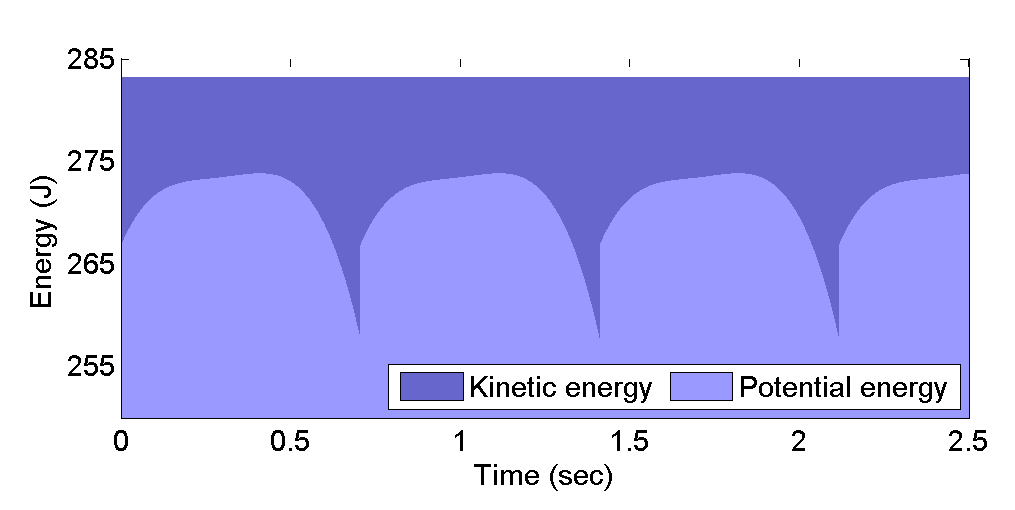
\includegraphics[width=1.0\columnwidth]{energy_cg2d_slope_model}
      \caption{Energy of the shaped system is conserved.}
    \end{figure}    
  }
  %  \only<3>{
  %    \includemedia[
  %      width=1.0\columnwidth,
  %      height=0.5625\columnwidth,
  %      addresource=amber2d.mp4,
  %      activate=pageopen,
  %      flashvars={source=amber2d.mp4&loop=true&autoPlay=true}
  %    ]{}{}%VPlayer9.swf}
  %  }

  \only<3>{
    Energy shaping can be achieved using:
    \begin{align*}
      \argmin_{u \in \Rn}  \, &\uu^{T} \uu\\
      \mbox{s.t. } & \Aclf\argsqdq \uu \leq \bclf\argsqdq
    \end{align*}
    where
    \begin{align*}
      \Aclf = 2 \eta \Lie{\xgbar} \eta, &&
      \bclf = -\resclfparam \eta^{2} - 2\eta \Lie{\xfbar} \eta,
    \end{align*}
    with
    \begin{align*}
      \eta = T\argsqdq + U(\Psi\argsq) - \Eref.
    \end{align*}
  }

  \only<4>{
    \begin{figure}
      \centering
      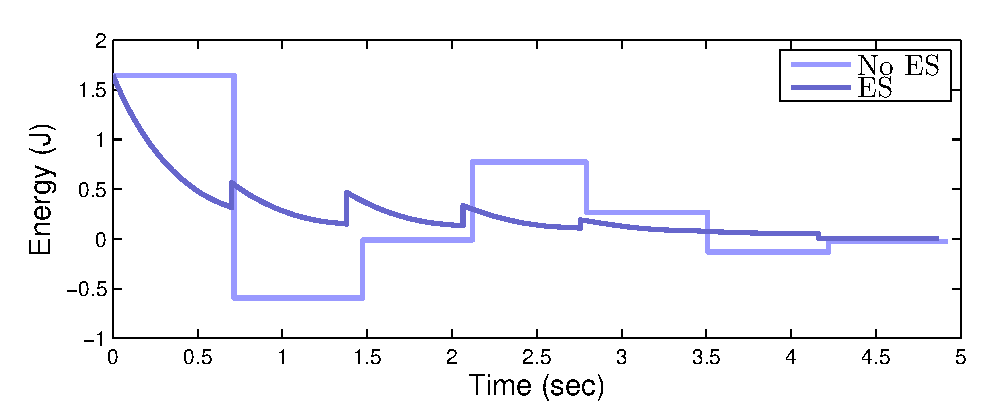
\includegraphics[width=1.0\columnwidth]{es_comparison_2link_conservative}
      \caption{Demonstration of energy shaping on 2-link biped.}
    \end{figure}
  }

  \only<5>{
    \begin{figure}
      \centering
      \includemedia[
        %width=1.0\columnwidth,
        %height=0.5625\columnwidth,
        width=1.0\columnwidth,
        height=0.5\columnwidth,
        addresource=cg2d_es.mp4,
        activate=pageopen,
        flashvars={source=cg2d_es.mp4&loop=true&autoPlay=true}
      ]{}{VPlayer9.swf}
      \caption{Energy shaping to stabilize to a gait from distant initial condition.}
    \end{figure}
  }

  \only<6> {
    \begin{figure}
      \centering
      \subfloat[Nominal system.]{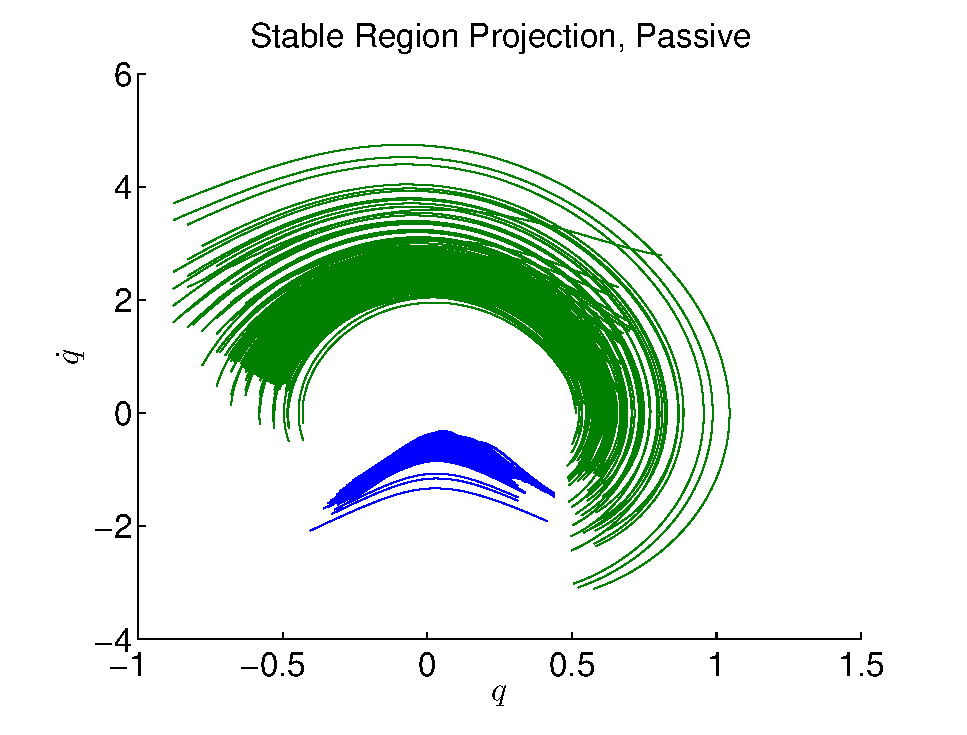
\includegraphics[width=.48\textwidth]{pp_eps_0}}
      \subfloat[Shaped system with $\resclfparam =
      \frac{1}{100}$.]{\includegraphics[width=.48\textwidth]{pp_eps_1_100}}
      \caption{Comparison of unshaped and shaped systems.}
    \end{figure}
  }

  \only<7> {
    \begin{figure}
      \centering
      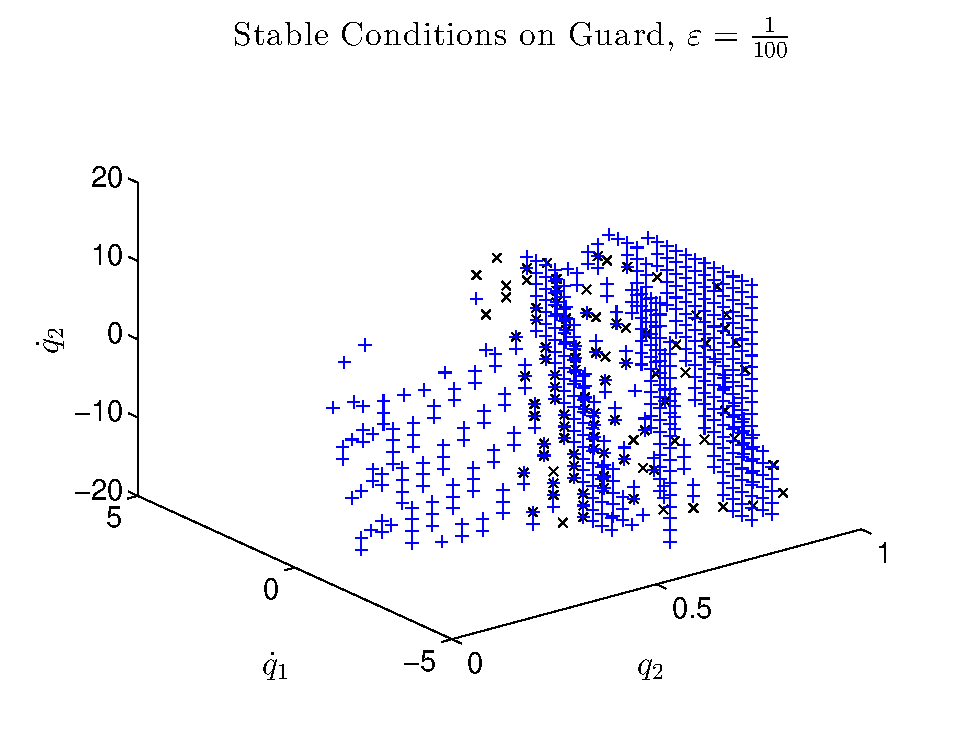
\includegraphics[height=.65\textheight]{poincare_cloud}
      \caption{A three-dimensional representation of the domain of attraction
        on the guard, comparing the unshaped and shaped system.}
    \end{figure}
  }
\end{frame}

\begin{frame}
  \frametitle{Example: 3-Link Biped}
  \only<1>{
    \begin{columns}
      \column{1.5in}
      Dynamic Model:
      \begin{align*}
        \M\argsq \ddq + \CG\argsqdq = \B\argsq \uu
      \end{align*}
      Control Law:
      \begin{align*}
        \vv\argsq& = \G\argsq - \G(\Psi\argsq)\\
        \vv_3\argsq& \ \  +\!= \ -k_{d} (\dot \vartheta_{T}^{a}\argsq)\\
        &\hspace{3.2em} -k_{p} (\vartheta_{T}^{a}\argsq - \vartheta_{T}^{d}\argsq)
      \end{align*}
      \column{1.5in}
      \begin{figure}
        \centering
        \def\svgwidth{1.0\columnwidth}
        \input{../figs/cg2d-3link-model.eps_latex}
        \vspace{-2em}
        \caption{3-link biped configuration.}
      \end{figure}
    \end{columns}
  }
  \only<2>{
    \begin{figure}
      \centering
      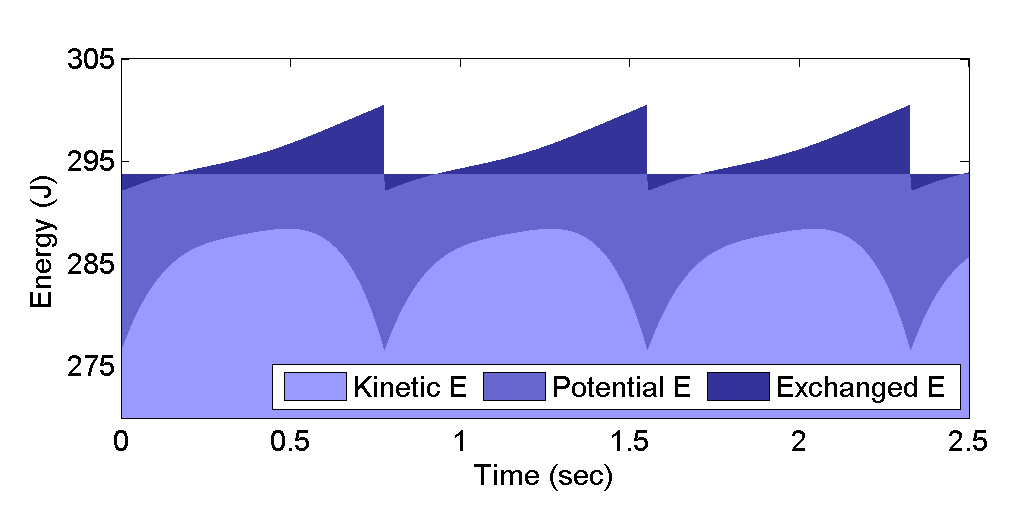
\includegraphics[width=1.0\columnwidth]{energy_conserved_cg2d_3link}
      \caption{The quantity, $\Ec\argsqdqW = T\argsqdq + V\argsq - \int_{0}^{t} F_{nc} \cdot \frac{d\q}{d\tau} d\tau$, is conserved.}
    \end{figure}
  }
  \only<3>{
    \begin{figure}
      \centering
      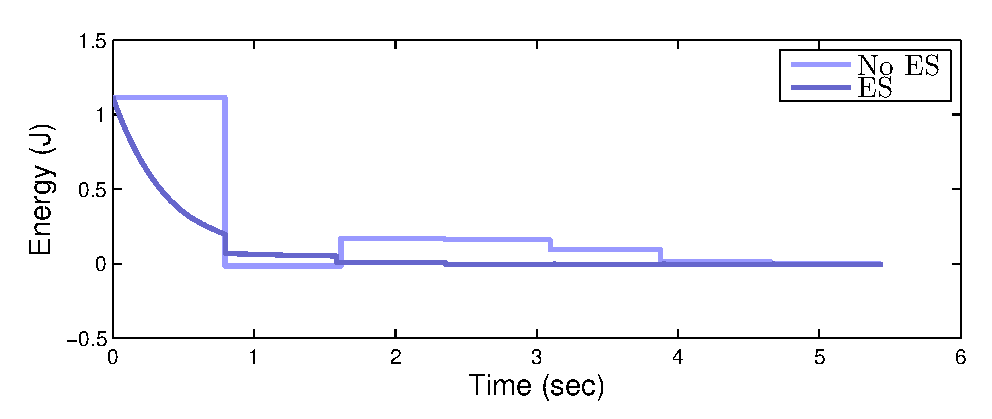
\includegraphics[width=1.0\columnwidth]{es_comparison_3link}
      \caption{Demonstration of energy shaping on 3-link biped.}
    \end{figure}
  }


  \only<4>{
    \begin{figure}
      \centering
      \includemedia[
        %width=1.0\columnwidth,
        %height=0.5625\columnwidth,
        width=1.0\columnwidth,
        height=0.5\columnwidth,
        addresource=3link_es.mp4,
        activate=pageopen,
        flashvars={source=3link_es.mp4&loop=true&autoPlay=true}
      ]{}{VPlayer9.swf}
      \caption{Energy shaping to stabilize to a gait from distant initial condition.}
    \end{figure}
  }

\end{frame}

\begin{frame}
  \frametitle{Multi-Domain Hybrid Systems}
  \begin{itemize}
  \item Complex hybrid systems are made by stitching together domains.
  \item Conserved energy is unique to each domain, i.e.,
    \begin{align*}
      E_0^{1} \to E_{0}^{2} \to \cdots \to E_{0}^{n-1} \to E_{0}^{n} \to E_{0}^{1} \to \cdots
    \end{align*}
  \item Each domain shapes to a specific conserved energy level.
  \end{itemize}
\end{frame}


\begin{frame}
  \frametitle{Example: 7-Link Biped with Feet}
  \only<1>{
    \blue{Appeared in {\bf Automatica}, Aug. 2014}
    \begin{columns}
      \column{1.5in}
      Dynamic Model:
      \begin{align*}
        \M\argsq \ddq + \CG\argsqdq = J^{T}\argsq \lambda + \B\argsq \uu
      \end{align*}
      \column{1.5in}
      \begin{figure}
        \centering
        \def\svgwidth{1.0\columnwidth}
        \input{../figs/cg2d-7link-model.eps_latex}
        \vspace{-2em}
        \caption{7-link biped configuration.}
      \end{figure}
    \end{columns}
  }

  \only<2>{
    \begin{block}{Spring--Damper Controller}
      \begin{align*}
        \vv_{\mathrm{SD}}\argsq = -\beta e^{-\rho \, h_{\mathrm{nst}}\argsq}
      \end{align*}
      where $\beta, \rho \in \R^{+}$ and $h_{\mathrm{nst}} : \Q \to \R$ is the height of the Nonstance toe.
      Used on
      \begin{itemize}
      \item Stance ankle\\
      \item Nonstance ankle\\
      \item Absolute torso angle\\
      \item Non-stance knee spring (only in double support)
      \end{itemize}
      \blue{Provides passivity-based control and toe-off.}
    \end{block}
  }

  \only<3>{
    \begin{block}{Scuffing Prevention Controller}
      \begin{align*}
        \vv_{\mathrm{SP}}\argsq = k_p \theta\argsq - k_d \dot \theta\argsqdq
      \end{align*}
      where $k_{p}, k_{d} \in \R^{+}$. Used on
      \begin{itemize}
      \item Nonstance ankle
      \end{itemize}
      \blue{Prevents the nonstance toe from colliding with the ground prematurely.}
    \end{block}
  }

\only<4>{
  \begin{figure}
    \centering
      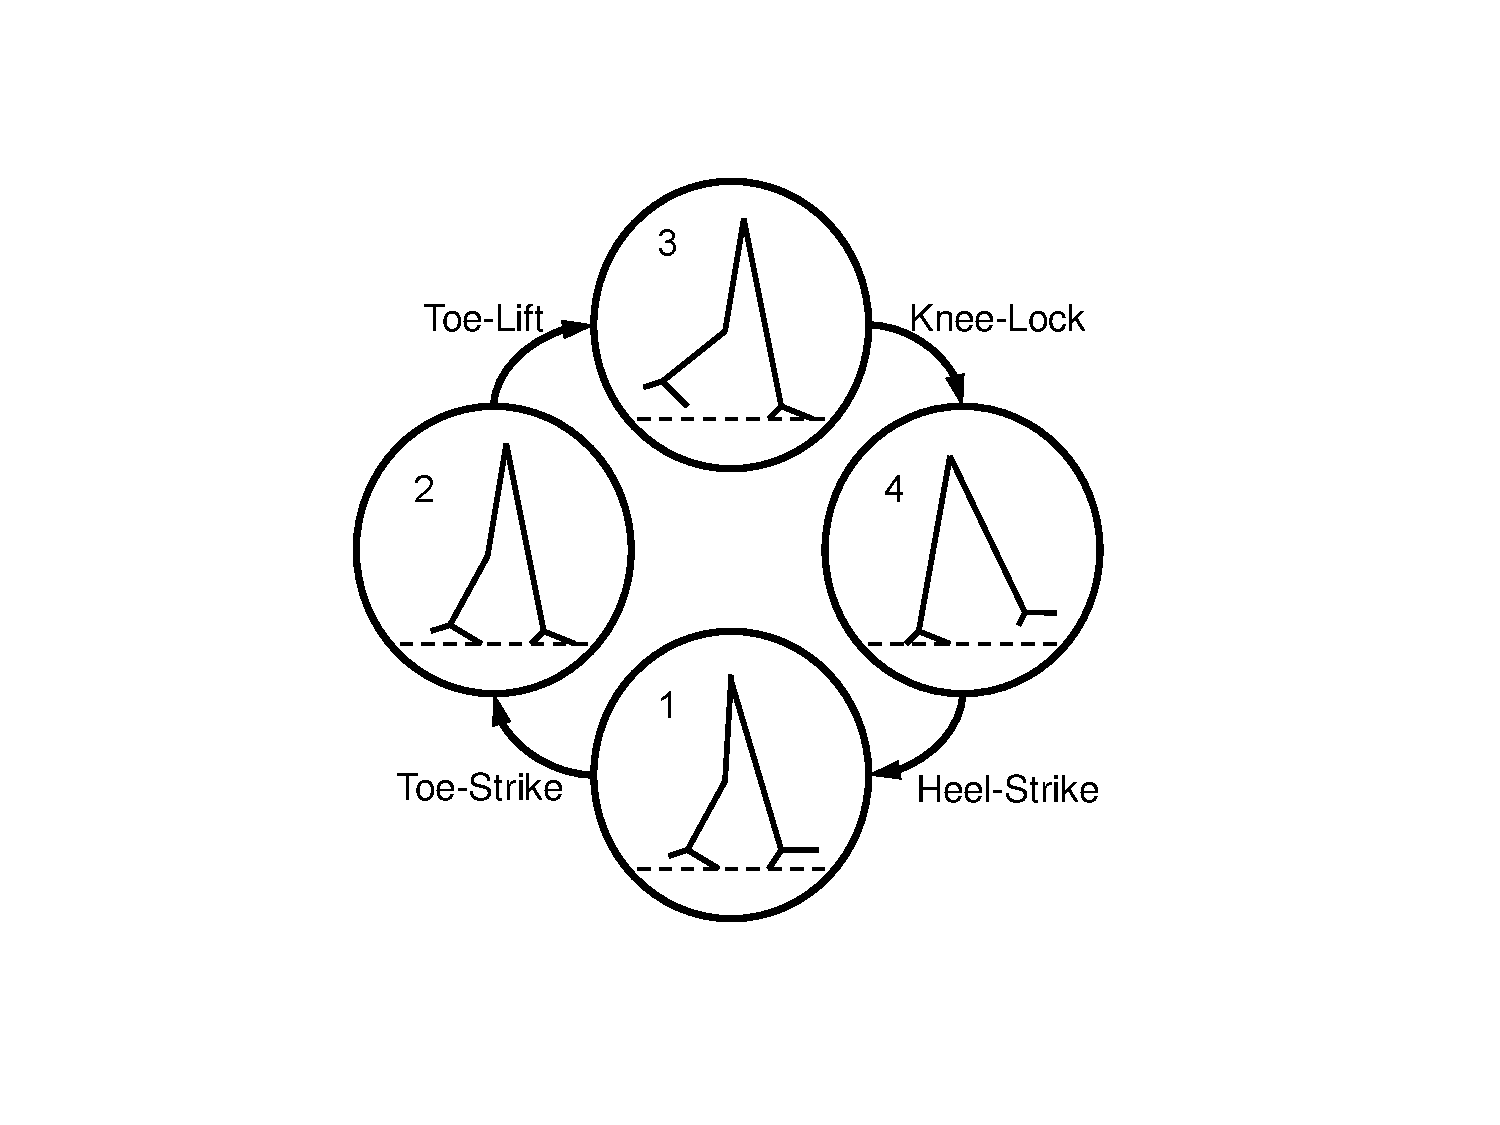
\includegraphics[height=.7\textheight]{domaingraph}
      \caption{The resulting gait traverses a four-domain directed graph.}
    \end{figure}
  }

  \only<5>{
    \begin{figure}
      \centering
      \includemedia[
        %width=1.0\columnwidth,
        %height=0.5625\columnwidth,
        width=1.0\columnwidth,
        height=0.5\columnwidth,
        addresource=7link_es.mp4,
        activate=pageopen,
        flashvars={source=7link_es.mp4&loop=true&autoPlay=true}
      ]{}{VPlayer9.swf}
      \caption{Energy shaping to stabilize to a gait.}
    \end{figure}
  }

  \only<6>{
    \begin{figure}
      \centering
      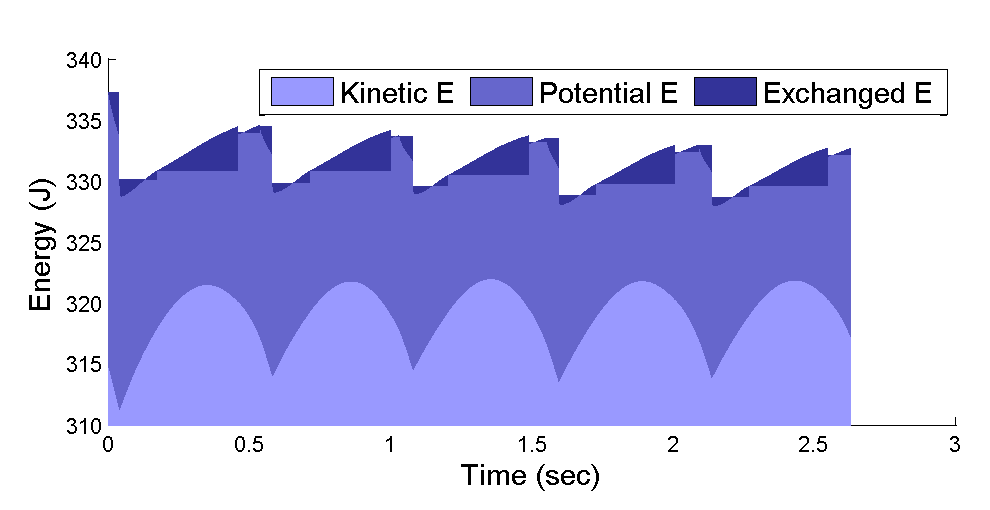
\includegraphics[width=1.0\columnwidth]{energy_conserved_7link}
      \caption{The quantity, $E_{0} \equiv T\argsqdq + U\argsq - \int_{0}^{t} F_{nc} \cdot \frac{d\q}{d\tau} d\tau$, is conserved.}
    \end{figure}
  }

  \only<7>{
    \begin{figure}
      \centering
      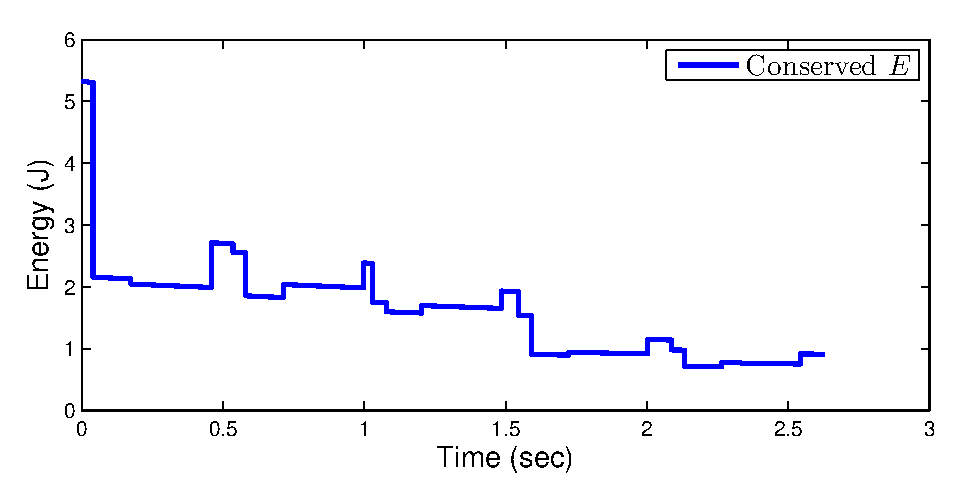
\includegraphics[width=1.0\columnwidth]{energy_conserved_7link_outline}
      \caption{The quantity, $E_{0} \equiv T\argsqdq + U\argsq - \int_{t_0}^{t} F_{nc} \cdot \frac{d\q}{d\tau} d\tau$, is conserved.}
    \end{figure}
  }
  \only<8>{
    \begin{figure}
      \centering
      \includemedia[
        %width=1.0\columnwidth,
        %height=0.5625\columnwidth,
        width=1.0\columnwidth,
        height=0.5\columnwidth,
        addresource=7link_noes.mp4,
        activate=pageopen,
        flashvars={source=7link_noes.mp4&loop=true&autoPlay=true}
      ]{}{VPlayer9.swf}
      \caption{Many steps on the limit cycle.}
    \end{figure}
  }
\end{frame}
}{}
\ifdefstring{\PRELIMSECE}{1}{\section{Questions}
\begin{frame}[t]
  \frametitle{Questions}
  \Large{Questions?}
\end{frame}
}{}

\end{document}
